\chapter{Реализация проекта для работы с базами данных}

Для проведения исследований необходимо описать интерфейс для работы с базами данных независимо от их типа и создать реализации для каждой участвующей базы данных, а именно PostgreSQL, Neo4j и ArangoDB.


\section{Описание интерфейса для работы с базами данных}

Для описания абстрактных методов без конкретной реализации в языке Java существуют интерфейсы. Интерфейс для работы с базой данных будет называться “Database” и он будет содержать следующие методы, необходимые для исследования:

\begin{itemize}
    \item init — метод для инициализации базы данных в случае необходимости подготовительных действий перед началом работы;
    \item clear — метод для очистки базы данных перед началом работы с новым графом;
    \item addNode — метод для добавления сущности (вершины графа);
    \item addEdge — метод для добавления отношения (ребро графа);
    \item addGraph — метод для одновременного добавления сущностей и отношений, если такая возможность присутствует в базе данных;
    \item getByNodeAttribute — метод для извлечения данных на основе атрибутов сущности (вершины графа);
    \item getByEdgeAttribute — метод для извлечения данных на основе атрибутов отношения (ребра графа);
    \item getShortestPath — метод для извлечения кратчайшего пути между двумя вершинами;
    \item getNearestNeighbors — метод для извлечения ближайших соседей к вершине на указанном уровне.
\end{itemize}

Дополнительно интерфейс “Database” расширяет интерфейс “AutoCloseable” для унаследования метода close в котором принято закрывать активные подключение к базам данных для правильной работы с ресурсами языка Java.


\section{Реализация интерфейса для PostgreSQL}

Для создания реляционной базы данных PostgreSQL на локальной машине используется Docker-образ “postgres” с переопределенным портом для подключения, выделенным одним процессором и настройками пользователя и базы данных.

\begin{figure}[ht!]
    \center
    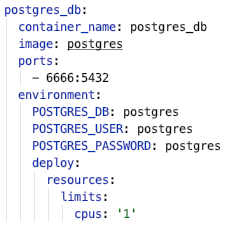
\includegraphics [scale=0.7] {my_folder/myimg//4}
    \caption{Настройки для запуска PostgreSQL в Docker-контейнере}
\end{figure}

Для подключения к созданной базе данных PostgreSQL в методе init класса “PostgresImpl” используются указанные в Docker-файле пользователь и база данных. При подключении в переменные класса сохраняются объекты подключение и состояния подключения к базе данных, для дальнейшего использования их в методах класса.


\section{Реализация интерфейса для Neo4j}

Для создания графовой базы данных Neo4j на локальной машине используется Docker-образ “neo4j” с предопределенными портами для подключения, выделенным одним процессором и настройками пользователя.

\begin{figure}[ht!]
    \center
    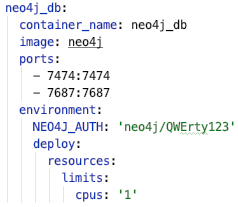
\includegraphics [scale=0.7] {my_folder/myimg//5}
    \caption{Настройки для запуска Neo4j в Docker-контейнере}
\end{figure}

Для подключения к созданной базе данных Neo4j в методе init класса “Neo4jImpl” используется указанный в Docker-файле пользователь. При подключении в переменные класса сохраняются объекты драйвера и сессии подключения к базе данных, для дальнейшего использования их в методах класса.


\section{Реализация интерфейса для ArangoDB}

Для создания мультимодельной базы данных ArangoDB на локальной машине используется Docker-образ “arangodb” с переопределенным портом для подключения, выделенным одним процессором и отключенной аутентификацией.

\begin{figure}[ht!]
    \center
    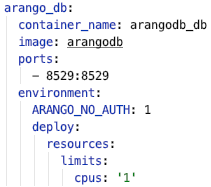
\includegraphics [scale=0.7] {my_folder/myimg//6}
    \caption{Настройки для запуска ArangoDB в Docker-контейнере}
\end{figure}

Для подключения к созданной базе данных ArangoDB в методе init класса “ArangoDBImpl” в переменные класса сохраняются объекты базы данных и графа, для дальнейшего использования их в методах класса.


\section{Создание интерфейса для логирования времени выполнения операций}

Для измерения времени выполнения каждой операции нужна ещё одна реализация интерфейса “Database”. Эта реализация не будет привязана к конкретной базе данных, она будет реализовывать шаблон делегирования. Это значит, что класс “LoggableDatabaseImpl” будет в конструкторе получать и сохранять реализацию интерфейса “Database” и в каждом методе передавать ей управление замеряя время до и после выполнения операции.


\section{Итоговая структура проекта для работы с базами данных}

Для проведения сравнения качества работы различных типов баз данных на классических графовых задачах был описан интерфейс “Database” для работы с базами данных независимо от их типа и созданы реализации для каждой базы данных, а именно “PostgresImpl”, “Neo4jImpl” и “ArangoDBImpl”, а так же создана реализация “ LoggableDatabaseImpl” для замера времени выполнения каждого метода, описанного в интерфейсе “Database”.

\begin{figure}[ht!]
    \center
    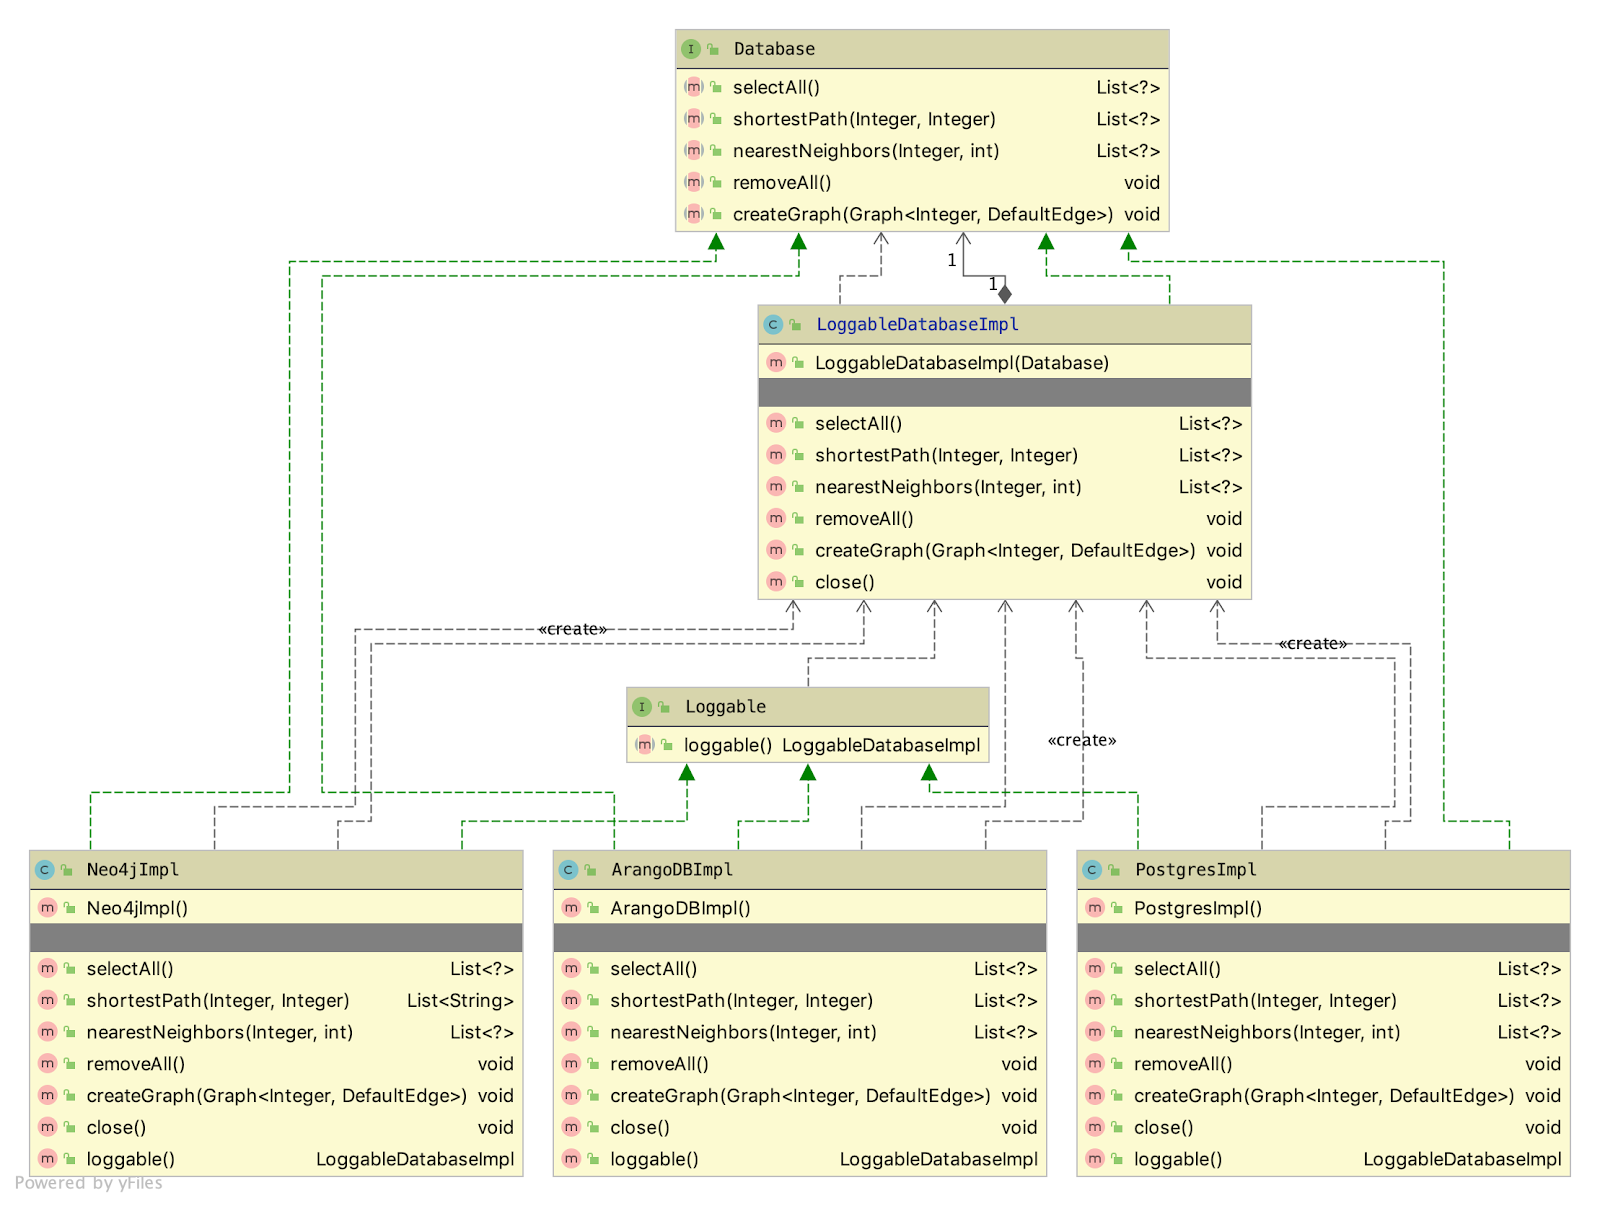
\includegraphics [scale=0.27] {my_folder/myimg//7}
    \caption{Структура проекта для работы с базами данных}
\end{figure}

%% Вспомогательные команды - Additional commands
%
%\newpage % принудительное начало с новой страницы, использовать только в конце раздела
%\clearpage % осуществляется пакетом <<placeins>> в пределах секций
%\newpage\leavevmode\thispagestyle{empty}\newpage % 100 % начало новой страницы